%% ============================================================
%% OpenDataCopilot -- Poster scientifique A0 portrait v2
%% Master 2 Data Science MIASHS -- Université Paul Valéry Montpellier
%% ============================================================
\documentclass[a0paper,portrait,25pt]{tikzposter}

%% ── Encodage & polices ──────────────────────────────────────
\usepackage[utf8]{inputenc}
\usepackage[T1]{fontenc}
\usepackage{lmodern}
\usepackage{bm}

%% ── TikZ & graphiques ───────────────────────────────────────
\usepackage{tikz}
\usetikzlibrary{shapes,arrows.meta,positioning,calc,fit,backgrounds}
\usepackage{pgfplots}
\pgfplotsset{compat=1.18}
\usepackage{graphicx}

%% ── Tableaux ────────────────────────────────────────────────
\usepackage{booktabs}
\usepackage{tabularx}
\usepackage{array}
\usepackage{colortbl}   % \rowcolor dans les tableaux

%% ── Boîtes colorées ─────────────────────────────────────────
\usepackage{tcolorbox}
\tcbuselibrary{skins}

%% ── Couleurs ────────────────────────────────────────────────
\usepackage{xcolor}
\definecolor{primary}{RGB}{44,62,80}
\definecolor{secondary}{RGB}{52,152,219}
\definecolor{accent}{RGB}{39,174,96}
\definecolor{alert}{RGB}{231,76,60}
\definecolor{orangecol}{RGB}{230,126,34}
\definecolor{lightbg}{RGB}{248,249,250}
%% Couleurs lignes tableau
\definecolor{rowred}{RGB}{253,235,235}
\definecolor{rowblue}{RGB}{232,244,253}
\definecolor{rowgreen}{RGB}{232,250,237}
\definecolor{roworange}{RGB}{254,243,228}
\definecolor{rowheader}{RGB}{44,62,80}

%% ── Divers ──────────────────────────────────────────────────
\usepackage{amssymb}
\usepackage{enumitem}
\setlist[itemize]{leftmargin=1.4em, itemsep=0.15em, topsep=0.3em}

%% ── Thème tikzposter ────────────────────────────────────────
\usetheme{Simple}
\usecolorstyle[colorOne=primary, colorTwo=secondary, colorThree=accent]{Default}
\tikzposterlatexaffectionproofoff
%% Fond blanc
\colorlet{backgroundcolor}{secondary!8}
%% Titres des blocks en noir (visible sur fond blanc)
\colorlet{blocktitlefgcolor}{black}

%% ── Styles TikZ globaux ─────────────────────────────────────
\tikzset{
  rbox/.style={rectangle, draw=primary!60, rounded corners=4pt,
               minimum width=5cm, minimum height=1.1cm,
               align=center, font=\small},
  arr/.style={-{Stealth[length=5pt,width=4pt]}, thick, color=primary!70},
}

%% ── Style tcolorbox réutilisable ────────────────────────────
\tcbset{
  badge/.style={
    colback=#1!15, colframe=#1, boxrule=1.5pt,
    arc=6pt, left=4pt, right=4pt, top=3pt, bottom=3pt,
  },
  recommande/.style={
    colback=accent!12, colframe=accent, boxrule=2pt,
    arc=8pt, left=8pt, right=8pt, top=6pt, bottom=6pt,
    title={\large\bfseries\color{primary} Syst\`eme Recommand\'e},
    colbacktitle=accent!30, coltitle=primary,
  },
}

%% ============================================================
%%  TITRE
%% ============================================================
\title{\parbox{0.90\linewidth}{\centering
  \large\textbf{OpenDataCopilot : Chatbot RAG Multi-Domaines}\\[0.3em]
  \normalsize Sant\'e Publique \& Pollution Atmosph\'erique --
  Comparaison de 4~Architectures RAG, 3~LLMs et 4~Embeddings}}
\author{\small J\'er\^ome ADJIMON}
\institute{\small Master 2 Data Science MIASHS --
           Universit\'e Paul Val\'ery Montpellier~3 \quad
           jerome.vitoff@etu.umontpellier.fr}

%% ============================================================
\begin{document}
\maketitle

\begin{columns}

%% ============================================================
%% COLONNE 1 — 22%
%% ============================================================
\column{0.22}

\block{1.\ Contexte \& Enjeux}{
  \centering
  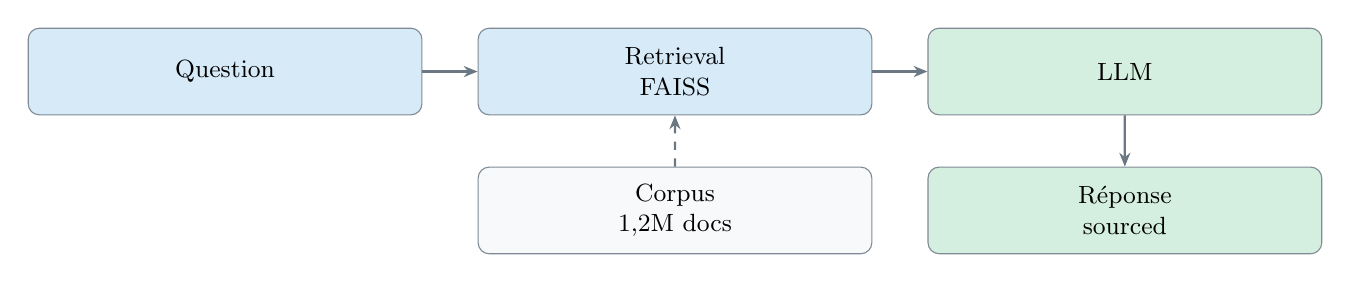
\begin{tikzpicture}[node distance=1cm and 1.1cm, scale=0.92]
    \node[rbox, fill=secondary!20] (q)   {Question};
    \node[rbox, fill=secondary!20, right=0.7cm of q]  (ret) {Retrieval\\FAISS};
    \node[rbox, fill=accent!20,    right=0.7cm of ret] (llm) {LLM};
    \node[rbox, fill=lightbg,      below=0.65cm of ret] (doc) {Corpus\\1{,}2M docs};
    \node[rbox, fill=accent!20,    right=0.7cm of doc]  (rep) {R\'eponse\\sourced};
    \draw[arr] (q)--(ret); \draw[arr] (ret)--(llm);
    \draw[arr,dashed] (doc)--(ret); \draw[arr] (llm)--(rep);
  \end{tikzpicture}

  \vspace{0.5cm}\raggedright
  \textbf{Probl\'ematique :}
  \begin{itemize}
    \item Donn\'ees publiques h\'et\'erog\`enes (sant\'e + air)
    \item Tol\'erance z\'ero aux hallucinations (contexte sant\'e)
    \item N\'ecessit\'e de donn\'ees temps r\'eel
  \end{itemize}

  \vspace{0.4cm}
  \begin{tabularx}{\linewidth}{@{}lX@{}}
    \textbf{Sources}   & SPF, ODISSE, Airparif, OpenAQ \\[0.2em]
    \textbf{P\'eriode} & 2019--2023 + temps r\'eel \\[0.2em]
    \textbf{Corpus}    & 1\,222\,802 documents \\[0.2em]
    \textbf{Dataset}   & 70 questions annot\'ees \\
  \end{tabularx}
}

\block{2.\ \'Etat de l'Art RAG}{

  \begin{tabularx}{\linewidth}{@{}lX@{}}
    \toprule
    \textbf{Technique} & \textbf{Avantage} \\
    \midrule
    Dense (FAISS)    & S\'emantique contextuelle \\[0.2em]
    Sparse (BM25)    & Correspondance mots-cl\'es \\[0.2em]
    \textbf{Hybride} & Combin\'e -- notre choix \\[0.2em]
    Reranking        & Pr\'ecision accrue \\
    \bottomrule
  \end{tabularx}

  \vspace{0.45cm}
  \textbf{Positionnement :} Aucun travail ant\'erieur ne compare
  syst\'ematiquement architectures RAG \emph{et} LLMs sur donn\'ees
  sant\'e publique fran\c{c}aises open data.

  \vspace{0.4cm}
  \textbf{Contribution :}
  \begin{itemize}
    \item 4 architectures valid\'ees / 70 questions
    \item 3 LLMs : GPT-3.5, Mistral~7B, Llama3
    \item 4 mod\`eles d'embeddings \'evalu\'es
    \item Prototype hybride temps r\'eel
  \end{itemize}
}


%% ============================================================
%% COLONNE 2 — 26%
%% ============================================================
\column{0.26}

\block{3.\ M\'ethodologie}{
  \centering
  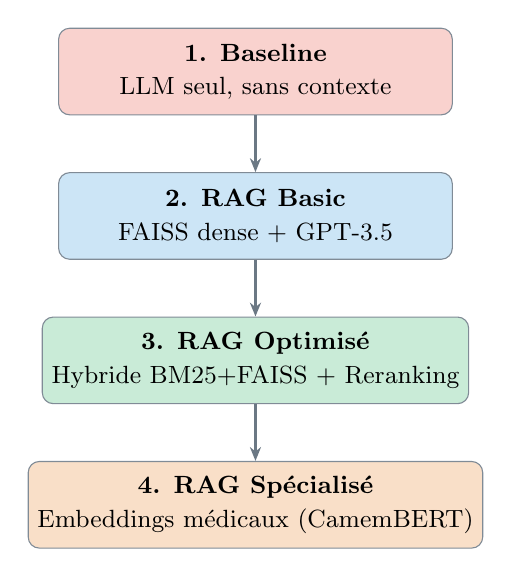
\begin{tikzpicture}[node distance=0.72cm]
    \node[rbox, fill=alert!25] (b1)
      {\textbf{1. Baseline}\\[0.12em]\small LLM seul, sans contexte};
    \node[rbox, fill=secondary!25, below=of b1] (b2)
      {\textbf{2. RAG Basic}\\[0.12em]\small FAISS dense + GPT-3.5};
    \node[rbox, fill=accent!25, below=of b2] (b3)
      {\textbf{3. RAG Optimis\'e}\\[0.12em]\small Hybride BM25+FAISS + Reranking};
    \node[rbox, fill=orangecol!25, below=of b3] (b4)
      {\textbf{4. RAG Sp\'ecialis\'e}\\[0.12em]\small Embeddings m\'edicaux (CamemBERT)};
    \draw[arr] (b1)--(b2); \draw[arr] (b2)--(b3); \draw[arr] (b3)--(b4);
  \end{tikzpicture}

  \vspace{0.45cm}\raggedright
  \textbf{Mod\`eles test\'es :}
  \begin{itemize}
    \item \textit{Embeddings :} OpenAI \texttt{text-embedding-3-small},
          Sentence-CamemBERT, Solon, CamemBERT-bio
    \item \textit{LLMs :} GPT-3.5-turbo, Mistral~7B (Ollama),
          Llama3~8B (Ollama), BioMistral~7B
    \item \textit{Reranker :} cross-encoder MiniLM-L-6
  \end{itemize}

  \vspace{0.3cm}
  \textbf{Protocole :} 70 questions $\times$ 4 architectures,
  \'evaluation automatis\'ee : qualit\'e, latence, co\^ut, hallucinations.
}

\block{4.\ Corpus \& \'Evaluation}{
  \centering
  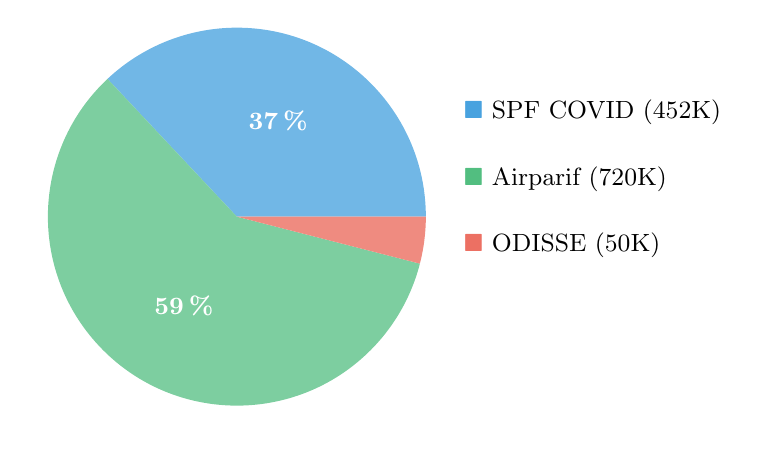
\begin{tikzpicture}[scale=1.2]
    \fill[secondary!70] (0,0) -- (2,0)
      arc[start angle=0, end angle=133.2, radius=2] -- cycle;
    \fill[accent!60] (0,0) -- ({2*cos(133.2)},{2*sin(133.2)})
      arc[start angle=133.2, end angle=345.6, radius=2] -- cycle;
    \fill[alert!65] (0,0) -- ({2*cos(345.6)},{2*sin(345.6)})
      arc[start angle=345.6, end angle=360, radius=2] -- cycle;
    \node[white,font=\small\bfseries] at ({1.1*cos(66.6)}, {1.1*sin(66.6)})  {37\,\%};
    \node[white,font=\small\bfseries] at ({1.1*cos(239.4)},{1.1*sin(239.4)}) {59\,\%};
    \node[right,font=\small] at (2.3, 1.1) {\textcolor{secondary!90}{$\blacksquare$}\ SPF COVID (452K)};
    \node[right,font=\small] at (2.3, 0.4) {\textcolor{accent!80}{$\blacksquare$}\ Airparif (720K)};
    \node[right,font=\small] at (2.3,-0.3) {\textcolor{alert!80}{$\blacksquare$}\ ODISSE (50K)};
  \end{tikzpicture}

  \vspace{0.2cm}
  \textbf{Total : 1\,222\,802 documents (2019--2023)}

  \vspace{0.4cm}\raggedright
  \begin{tabularx}{\linewidth}{@{}Xc@{}}
    \toprule
    \textbf{Cat\'egorie de questions} & \textbf{N} \\
    \midrule
    Sant\'e (COVID, vaccination, \'epid\'emio.)  & 30 \\[0.12em]
    Qualit\'e de l'air (NO$_2$, PM$_{10}$, O$_3$) & 20 \\[0.12em]
    Corr\'elations sant\'e--pollution             & 20 \\
    \midrule
    \textbf{Total}                               & \textbf{70} \\
    \bottomrule
  \end{tabularx}

  \vspace{0.3cm}
  \textbf{M\'etriques :} Qualit\'e (utilit\'e jury), pertinence FAISS,
  taux d'hallucination, latence, co\^ut/question.
}

\block{8.\ \'Evaluation Critique}{
  \textcolor{accent}{\textbf{R\'eussites :}}
  \begin{itemize}
    \item Comparaison rigoureuse 4 architectures / 3 LLMs
    \item 6 d\'ecouvertes scientifiques valid\'ees
    \item 0\,\% hallucination sur toutes architectures
    \item Prototype hybride temps r\'eel fonctionnel
  \end{itemize}

  \textcolor{orangecol}{\textbf{Difficult\'es :}}
  \begin{itemize}
    \item Bug Git : 2.65\,GB $\to$ 11\,MB (BFG, r\'esolu)
    \item Sp\'ecialisation m\'edicale inefficace ($-$5\,\%)
  \end{itemize}

  \textcolor{secondary}{\textbf{Apprentissages :}}
  Architecture RAG, \'evaluation LLM, Git avanc\'e,
  APIs open data, infrastructure Ollama locale.
}


%% ============================================================
%% COLONNE 3 — 26%
%% ============================================================
\column{0.26}

\block{5.\ R\'esultats -- Comparaison}{

  \centering
  %%  Tableau avec lignes colorées
  \setlength{\arrayrulewidth}{0.6pt}
  \begin{tabular}{@{}lcccc@{}}
    \toprule
    \rowcolor{rowheader}
    \textcolor{white}{\textbf{Architecture}} &
    \textcolor{white}{\textbf{Qualit\'e}} &
    \textcolor{white}{\textbf{Lat.}} &
    \textcolor{white}{\textbf{Co\^ut/Q}} &
    \textcolor{white}{\textbf{}} \\
    \midrule
    \rowcolor{rowred}
    Baseline           & 0.300 & 1.8\,s & \$0.006   & \textcolor{alert}{$\times$} \\[0.1em]
    \rowcolor{rowblue}
    RAG Basic          & 0.743 & 2.9\,s & \$0.091   & \textcolor{accent}{$\checkmark$} \\[0.1em]
    \rowcolor{rowblue}
    RAG Optimis\'e     & \underline{0.754} & 5.0\,s & \$0.103 & \textcolor{accent}{$\star$} \\[0.1em]
    \rowcolor{roworange}
    RAG Sp\'ecialis\'e & 0.706 & 9.4\,s & \$0.117   & \textcolor{orangecol}{$\times$} \\[0.1em]
    \rowcolor{rowgreen}
    \textbf{Mistral 7B}& \textbf{0.757} & \textbf{3.1\,s} & \textbf{\$0.0002} & \textcolor{accent}{$\star\star$} \\[0.1em]
    \rowcolor{rowgreen}
    Llama3 8B          & 0.760 & 4.5\,s & \$0.0002  & \textcolor{accent}{$\checkmark$} \\
    \bottomrule
  \end{tabular}

  \vspace{0.4cm}
  %% Badge 0% hallucination
  \begin{tcolorbox}[badge=accent, width=\linewidth]
    \centering\large
    \textbf{Hallucinations : 0\,\%} \quad $|$ \quad
    \textbf{Sources cit\'ees : 100\,\%}\\
    \small valid\'e sur 70 questions, 4 architectures
  \end{tcolorbox}

  \vspace{0.3cm}
  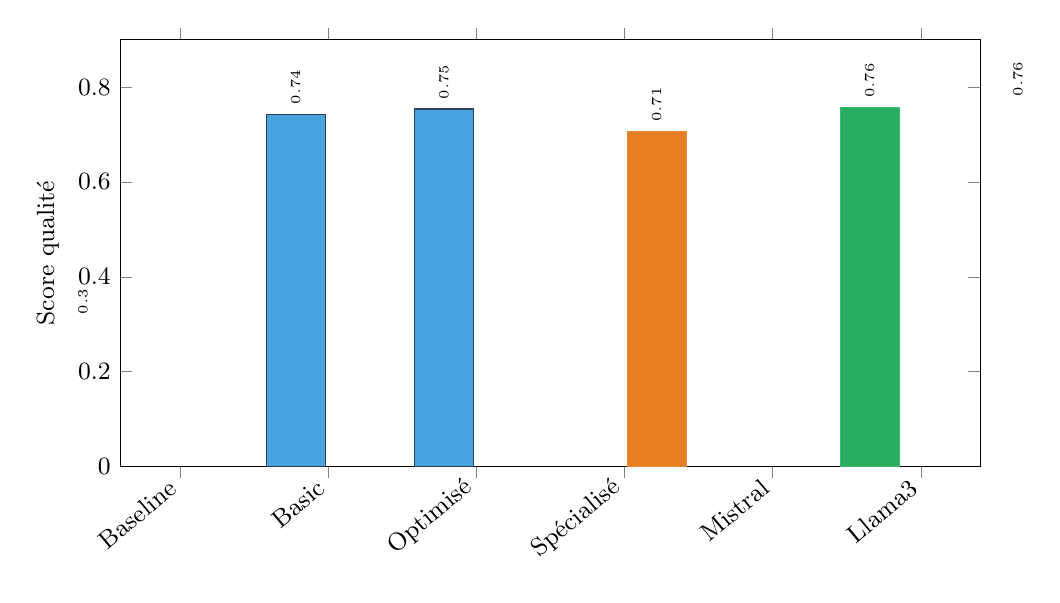
\begin{tikzpicture}
    \begin{axis}[
      ybar,
      width=12.5cm, height=7cm,
      ylabel={Score qualit\'e},
      ylabel style={font=\small},
      xtick={1,2,3,4,5,6},
      xticklabels={Baseline, Basic, Optimis\'e, Sp\'ecialis\'e, Mistral, Llama3},
      xticklabel style={rotate=40, anchor=east, font=\small},
      yticklabel style={font=\small},
      nodes near coords, nodes near coords style={font=\tiny, rotate=90, anchor=west},
      ymin=0, ymax=0.9,
      bar width=0.75cm,
      every axis plot/.style={fill=secondary!65, draw=primary!70},
      enlarge x limits=0.08,
    ]
    \addplot[fill=alert,        draw=alert!90]      coordinates {(1,.300)};
    \addplot[fill=secondary!90, draw=primary]       coordinates {(2,.743)(3,.754)};
    \addplot[fill=orangecol,    draw=orangecol!90]  coordinates {(4,.706)};
    \addplot[fill=accent,       draw=accent!90]     coordinates {(5,.757)(6,.760)};
    \end{axis}
  \end{tikzpicture}
}

\block{6.\ D\'ecouvertes Scientifiques}{

  \textbf{\textcolor{secondary}{1.\ Diversit\'e $>$ Volume}} :
  $+$114\,\% docs $=$ $+$18.9\,\% pertinence seulement

  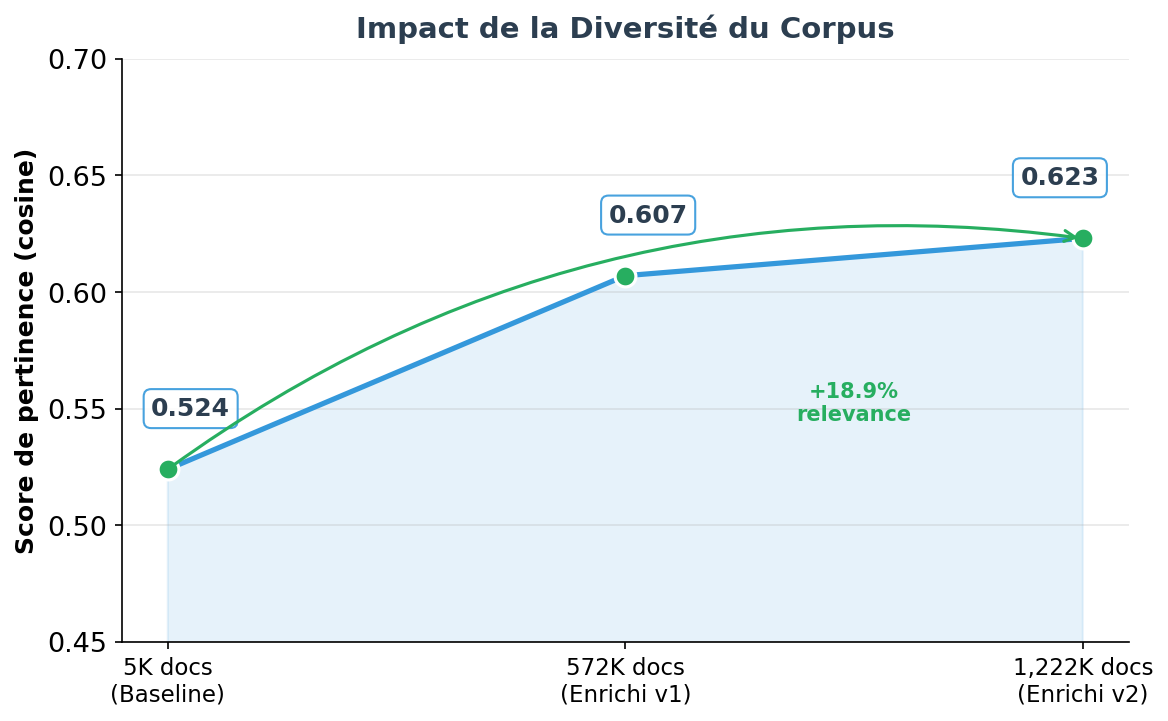
\includegraphics[width=\linewidth]{assets/graph_diversite.png}

  \vspace{0.1cm}
  \textbf{\textcolor{secondary}{2.\ Open-source comp\'etitif}} :
  Mistral~7B $\approx$ GPT-3.5, $\times$500 moins cher

  \vspace{0.1cm}
  \textbf{\textcolor{secondary}{3.\ Complexit\'e $\neq$ Performance}} :
  sur-ing\'enierie $-$6\,\% qualit\'e

  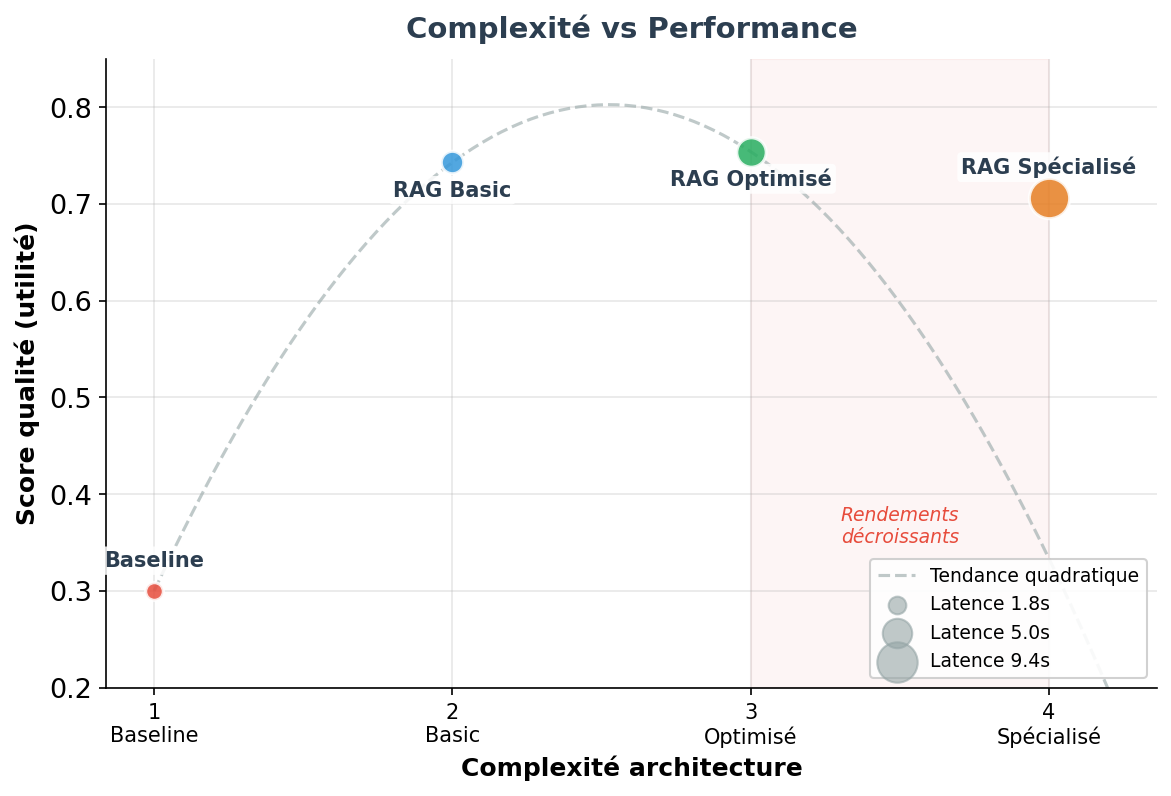
\includegraphics[width=\linewidth]{assets/graph_complexite.png}

  \vspace{0.1cm}
  \textbf{\textcolor{secondary}{4.\ T\^ache $>$ Domaine}} :
  OpenAI g\'en\'eraliste $>$ CamemBERT-bio ($-$78\,\%)

  \vspace{0.1cm}
  \textbf{\textcolor{secondary}{5.\ RAG = 0\,\% hallucination}} $\cdot$
  \textbf{\textcolor{secondary}{6.\ 20$\to$70 questions}} r\'ev\`ele les vraies performances

  \vspace{0.35cm}
  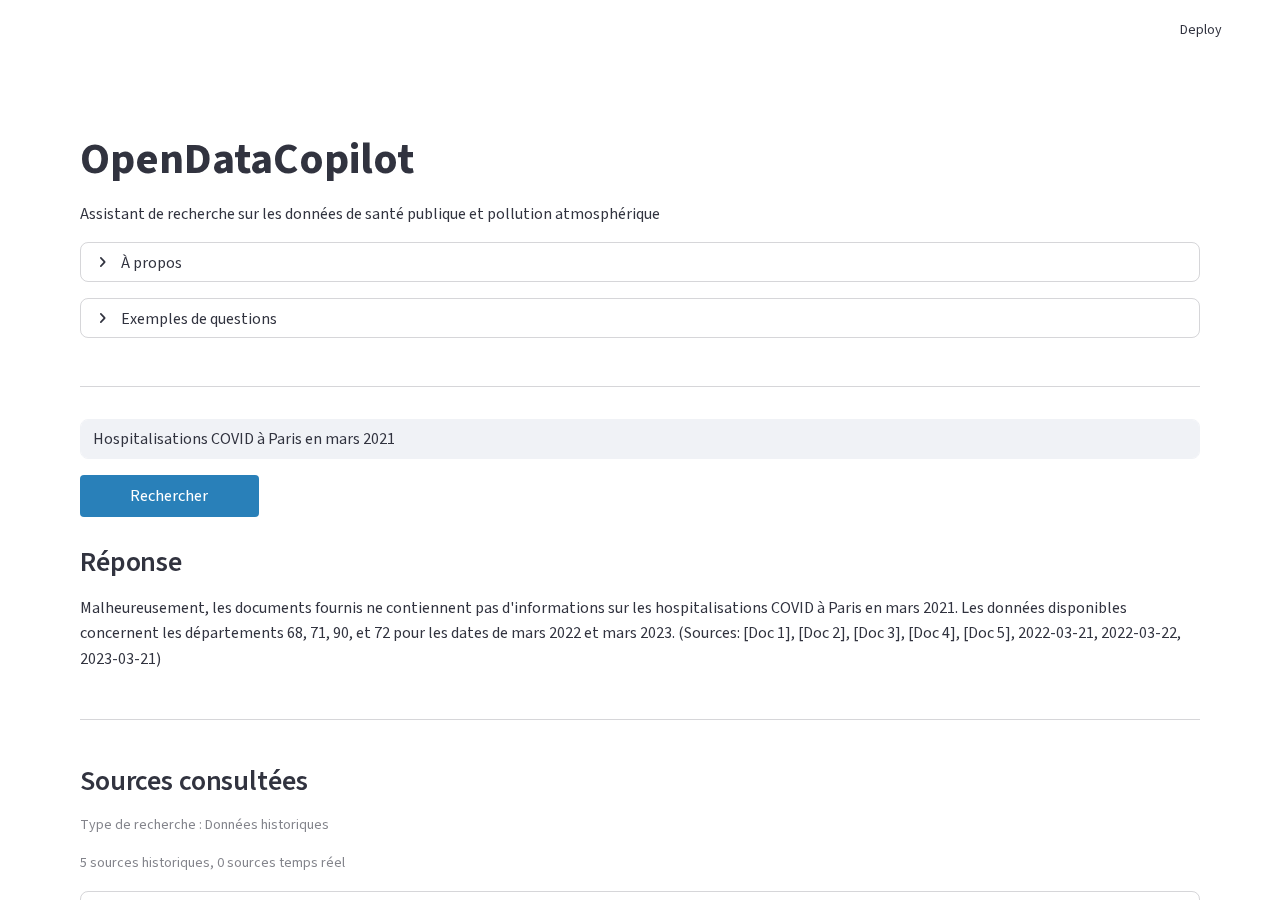
\includegraphics[width=\linewidth]{assets/06_question_sante_covid.png}
  \par{\small\textit{Sant\'e historique -- COVID hospitalisations}}

  \vspace{0.25cm}
  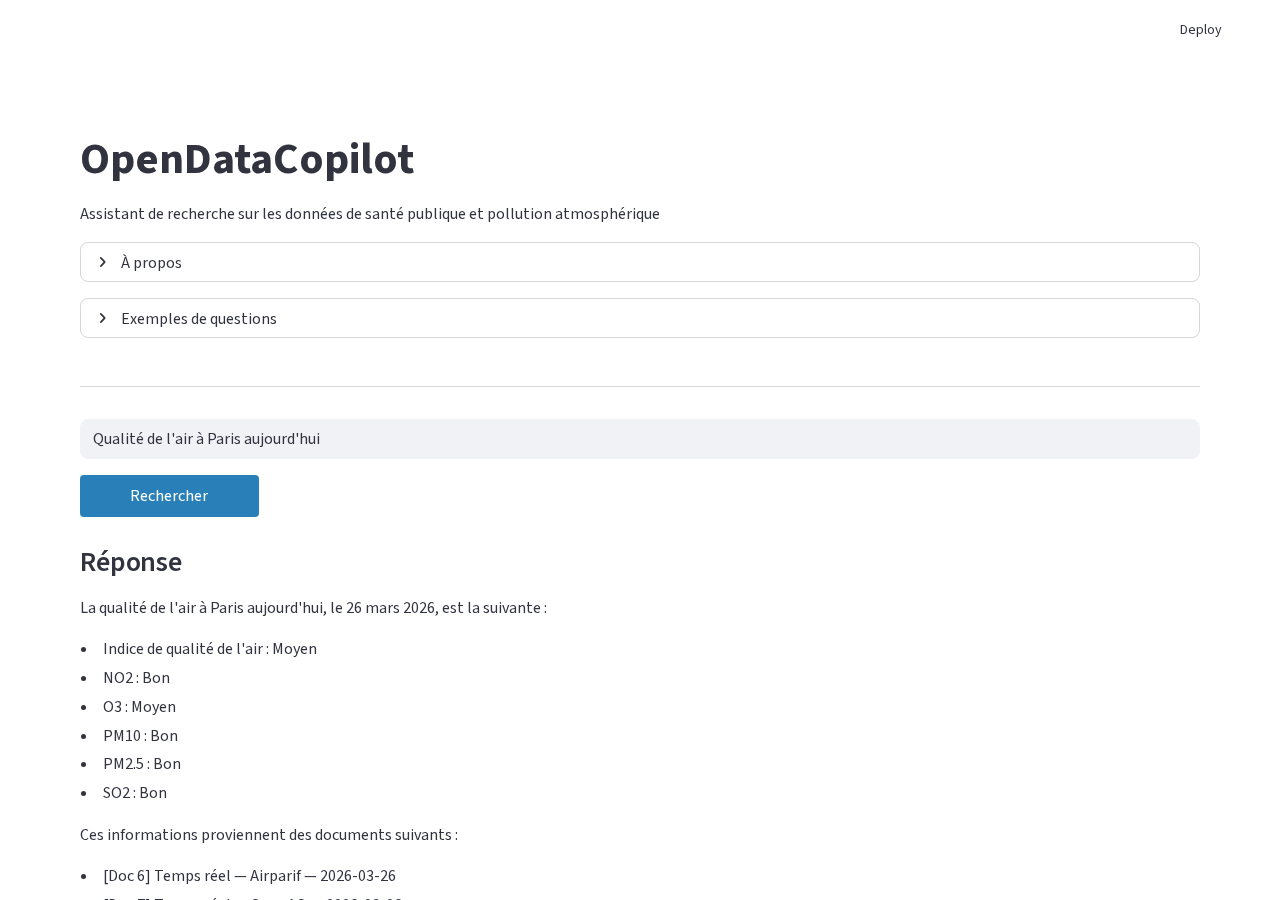
\includegraphics[width=\linewidth]{assets/03_temps_reel_air.png}
  \par{\small\textit{Qualit\'e de l'air temps r\'eel -- Paris}}
}


%% ============================================================
%% COLONNE 4 — 26%
%% ============================================================
\column{0.26}

\block{7.\ Prototype Hybride Temps R\'eel}{
  \centering
  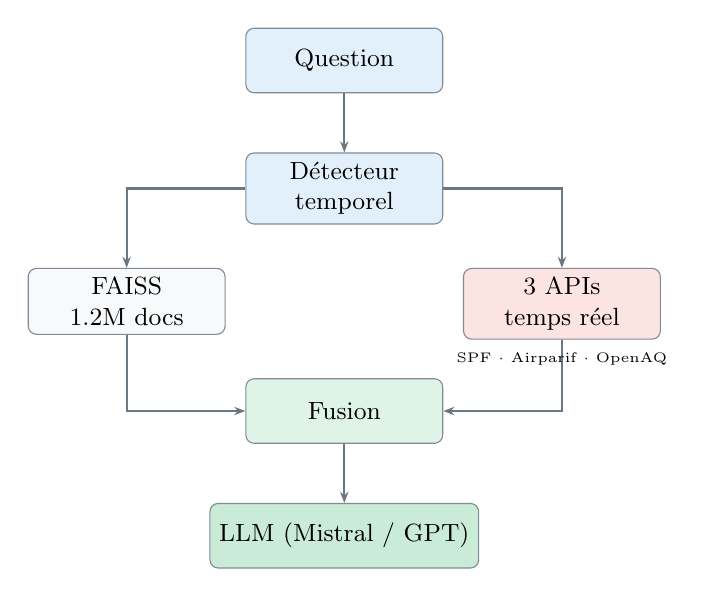
\begin{tikzpicture}[
    node distance=0.75cm and 1.2cm,
    fbox/.style={rectangle, draw=primary!60, fill=secondary!15, rounded corners=3pt,
                 minimum width=2.5cm, minimum height=0.82cm, align=center, font=\small},
    arr2/.style={-{Stealth[length=4pt]}, thick, color=primary!70}
  ]
    \node[fbox] (q)   {Question};
    \node[fbox, below=of q] (det) {D\'etecteur\\temporel};
    \node[fbox, fill=lightbg,  below left =0.55cm and 0.25cm of det] (hist) {FAISS\\1.2M docs};
    \node[fbox, fill=alert!15, below right=0.55cm and 0.25cm of det] (rt)   {3 APIs\\temps r\'eel};
    \node[fbox, fill=accent!15, below right=0.55cm and 0.25cm of hist] (fus) {Fusion};
    \node[fbox, fill=accent!25, below=of fus] (llm) {LLM (Mistral / GPT)};
    \draw[arr2] (q)--(det);
    \draw[arr2] (det)-|(hist); \draw[arr2] (det)-|(rt);
    \draw[arr2] (hist)|-(fus); \draw[arr2] (rt)|-(fus);
    \draw[arr2] (fus)--(llm);
    \node[font=\tiny, below=0.04cm of rt]{SPF $\cdot$ Airparif $\cdot$ OpenAQ};
  \end{tikzpicture}

  \vspace{0.3cm}\raggedright
  \begin{tabularx}{\linewidth}{@{}Xcc@{}}
    \toprule
    \textbf{Composant}          & \textbf{Tests} & \textbf{OK} \\
    \midrule
    D\'etection temporelle      & 19/19 & \textcolor{accent}{$\checkmark$} \\[0.1em]
    APIs temps r\'eel           & 3/3   & \textcolor{accent}{$\checkmark$} \\[0.1em]
    Cache ($\times$4 perf.)     & pass  & \textcolor{accent}{$\checkmark$} \\[0.1em]
    Fusion hist.\ + RT          & 3/3   & \textcolor{accent}{$\checkmark$} \\[0.1em]
    Interface Streamlit         & pass  & \textcolor{accent}{$\checkmark$} \\
    \bottomrule
  \end{tabularx}

  \vspace{0.35cm}\centering
  %% Grande capture : pollution actuelle
  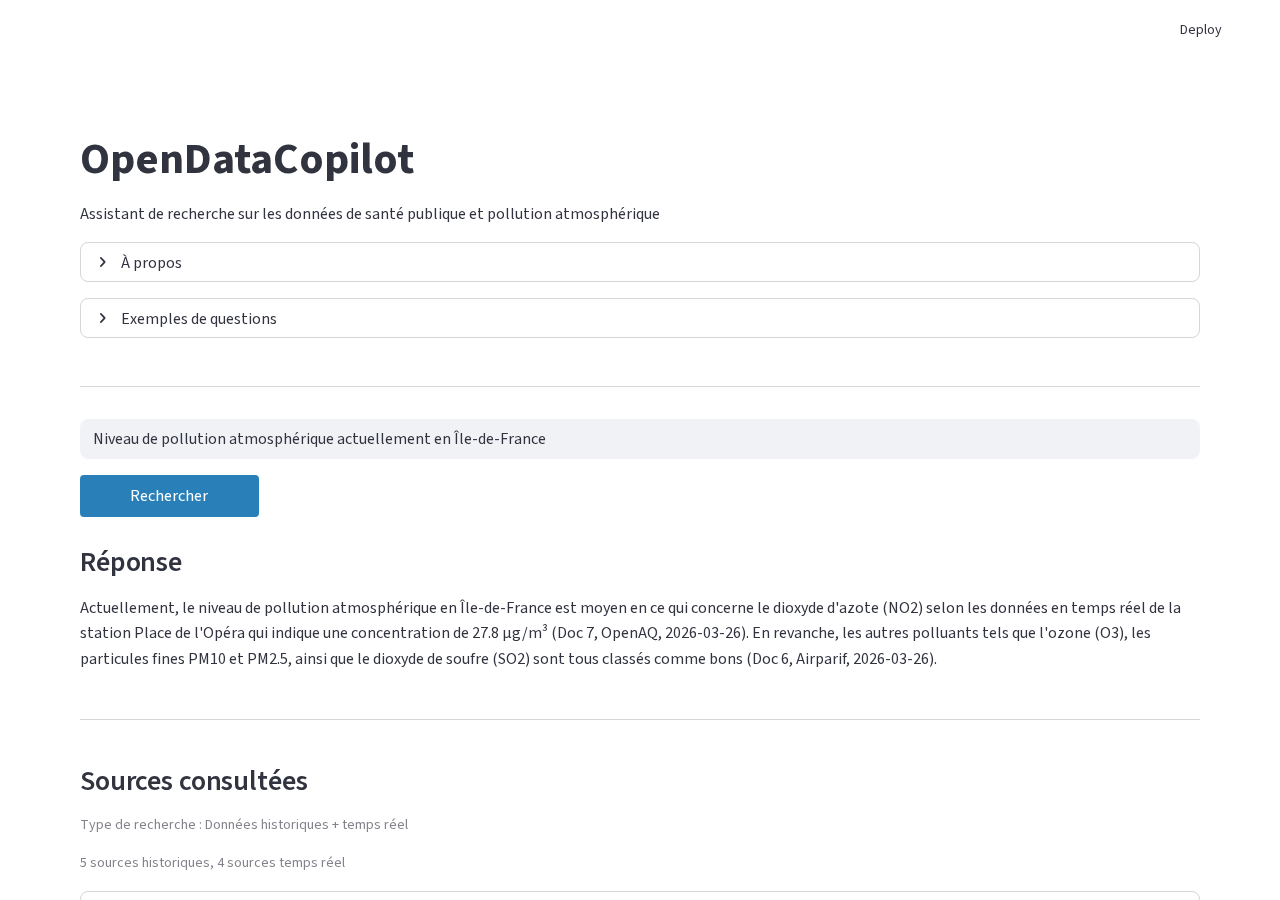
\includegraphics[width=\linewidth]{assets/05_pollution_actuelle.png}
  \par{\small\textit{Pollution temps r\'eel -- \^Ile-de-France}}

  \vspace{0.3cm}
  %% Capture hybride (domaine crois\'e)
  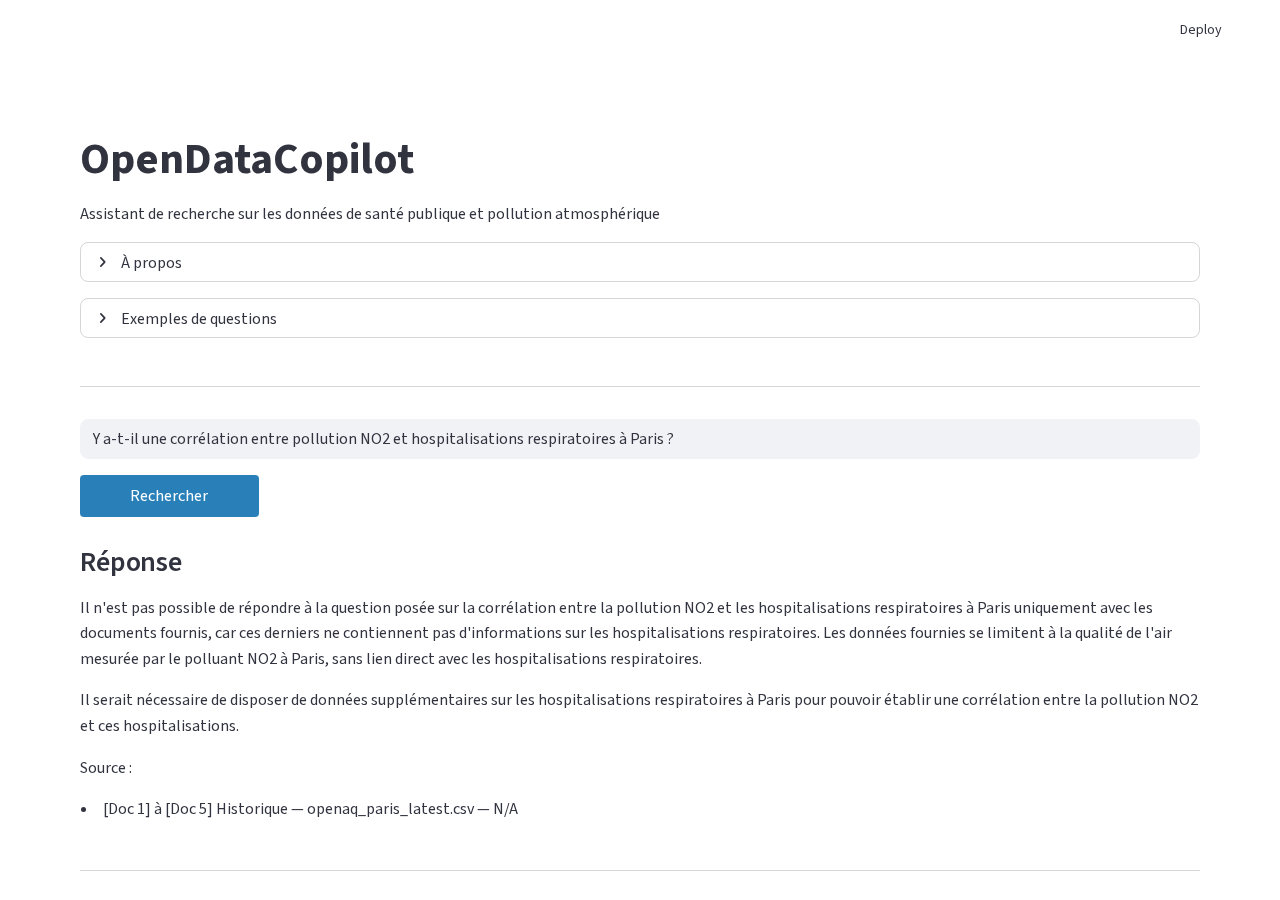
\includegraphics[width=\linewidth]{assets/07_question_hybride_sante_pollution.png}
  \par{\small\textit{Fusion sant\'e + pollution (corr\'elation NO$_2$)}}

  \vspace{0.3cm}
  %% Badge + capture hors base
  \begin{tcolorbox}[badge=alert, width=\linewidth]
    \centering\small\textbf{Validation 0\,\% hallucination}\\
    Question hors base~$\to$ aveu d'ignorance
  \end{tcolorbox}
  \vspace{0.2cm}
  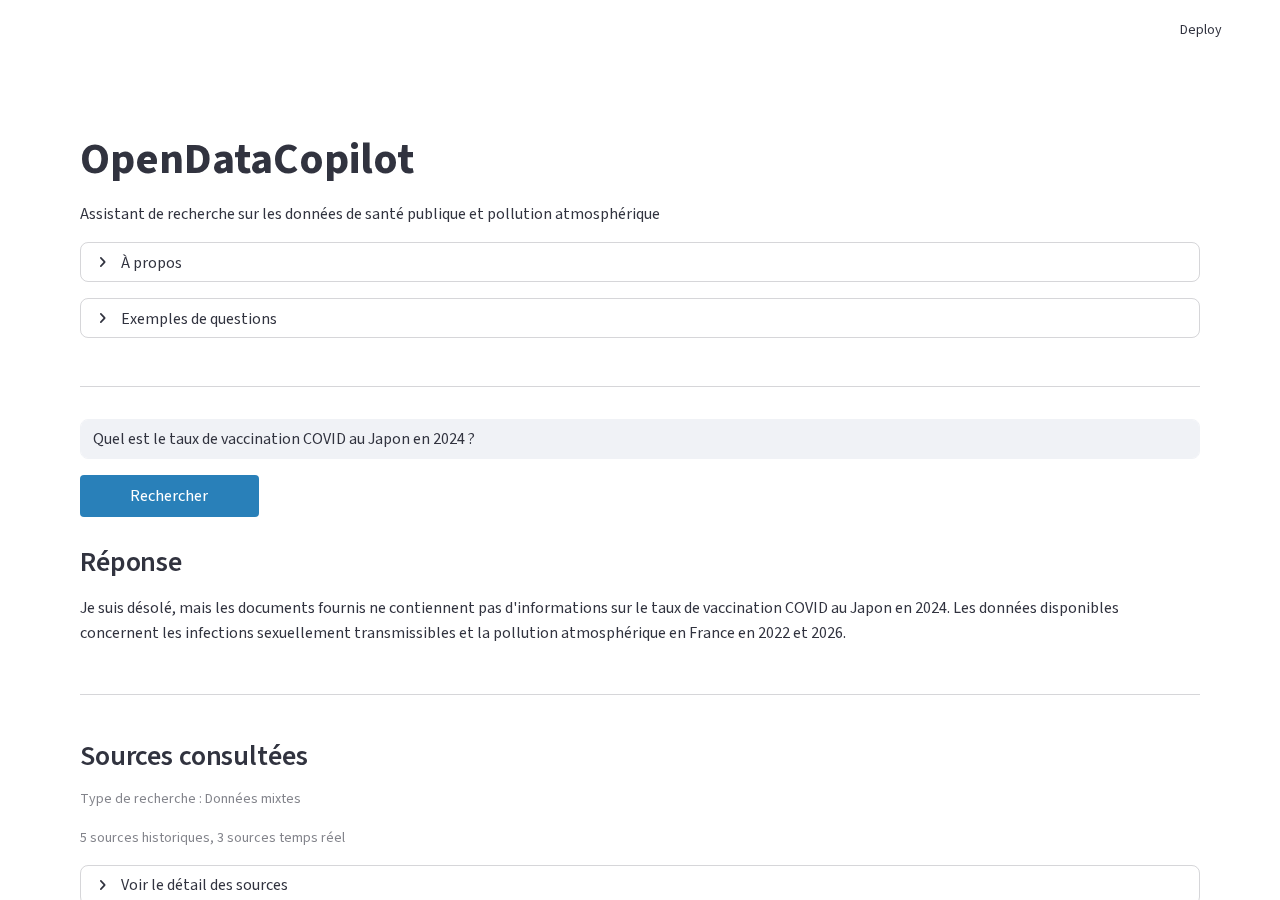
\includegraphics[width=0.95\linewidth]{assets/08_question_hors_base.png}
  \par{\small\textit{Japon 2024 : syst\`eme honnête, pas de confabulation}}
}

\block{9.\ Perspectives}{
  \textbf{Court terme} \textcolor{accent}{(\checkmark)} :
  Prototype + interface Streamlit\\[0.25em]
  \textbf{Moyen terme :}
  D\'eploiement Docker, fine-tuning Mistral-FR\\[0.25em]
  \textbf{Long terme :}
  Multi-hop reasoning, extension domaines

  \vspace{0.5cm}
  %% Encadré Système Recommandé
  \begin{tcolorbox}[recommande]
    \centering
    \large\textbf{RAG Optimis\'e + Mistral~7B}\\[0.4em]
    \normalsize
    Qualit\'e : \textbf{0.757} \quad
    Co\^ut : \textbf{\$0.0002/Q}\\[0.2em]
    Latence : \textbf{3.1\,s} \quad
    Hallucinations : \textbf{0\,\%}\\[0.2em]
    \small D\'eploiement local RGPD-compliant
  \end{tcolorbox}
}

\end{columns}

\end{document}
